\begin{figure}[h]
	\centering
	\setlength{\resLen}{1.55in}
	\addtolength{\tabcolsep}{-3.5pt}
	\begin{tabular}{cccc}
		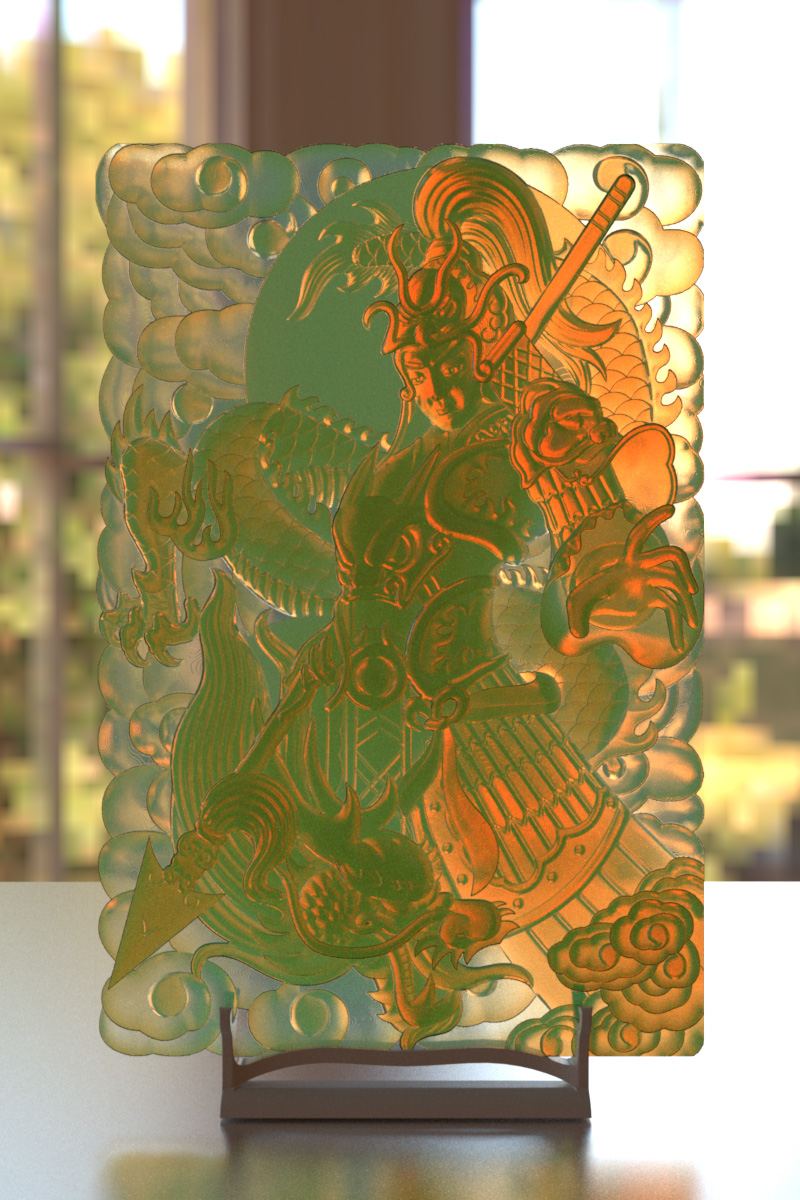
\includegraphics[width=\resLen]{layeredbsdf/results/zhaoyun_bg1_1.jpg} &
		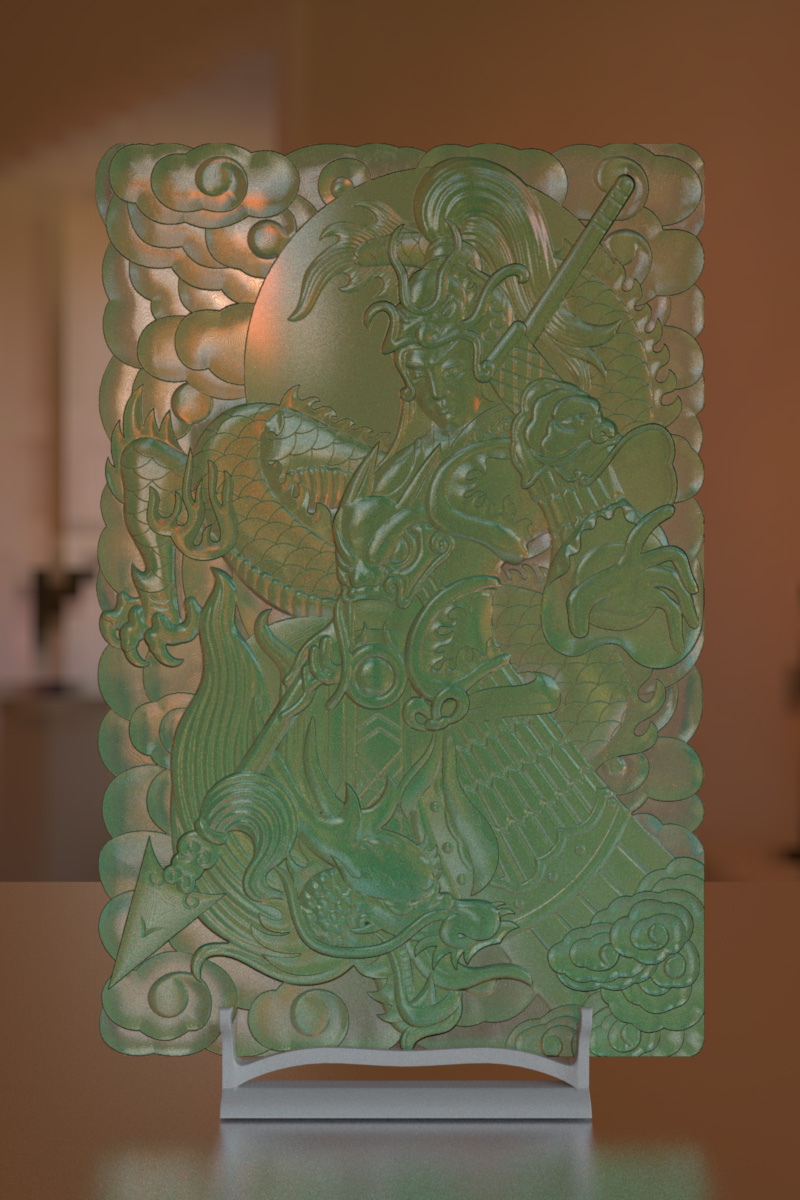
\includegraphics[width=\resLen]{layeredbsdf/results/zhaoyun_bg1_2.jpg} &
		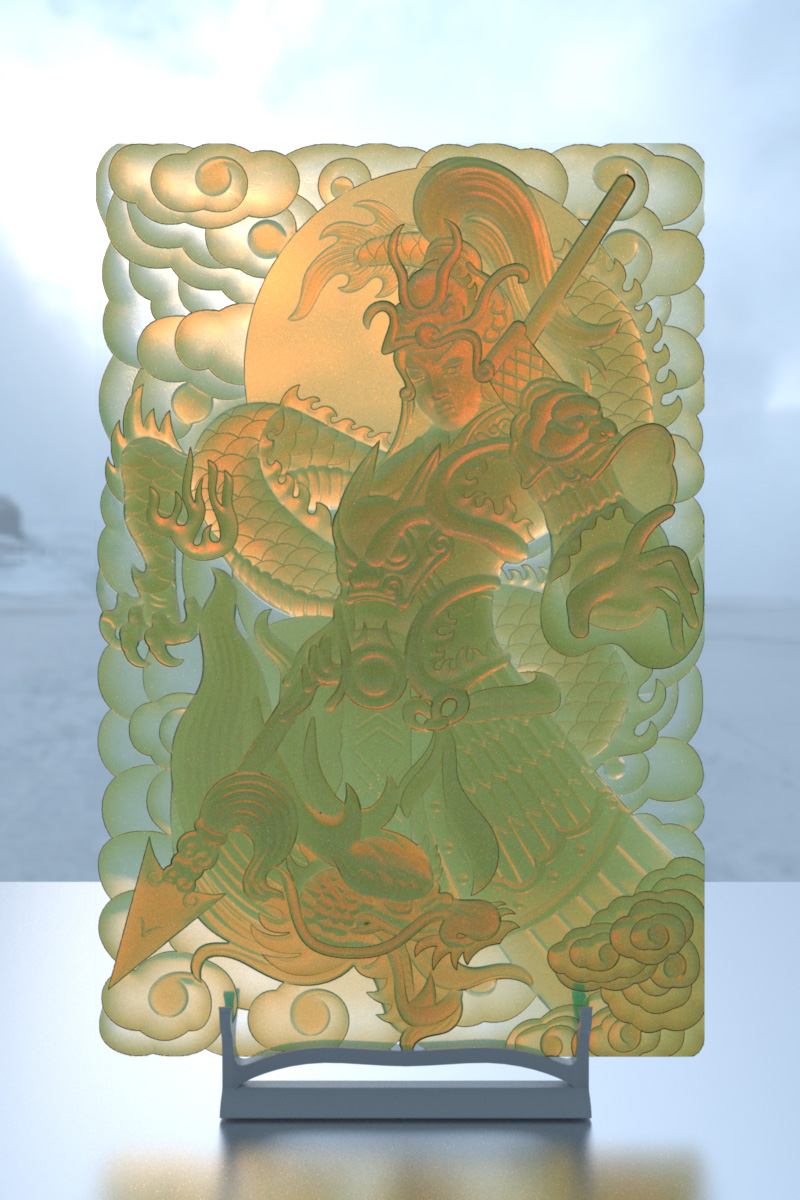
\includegraphics[width=\resLen]{layeredbsdf/results/zhaoyun_bg2_1.jpg} &
		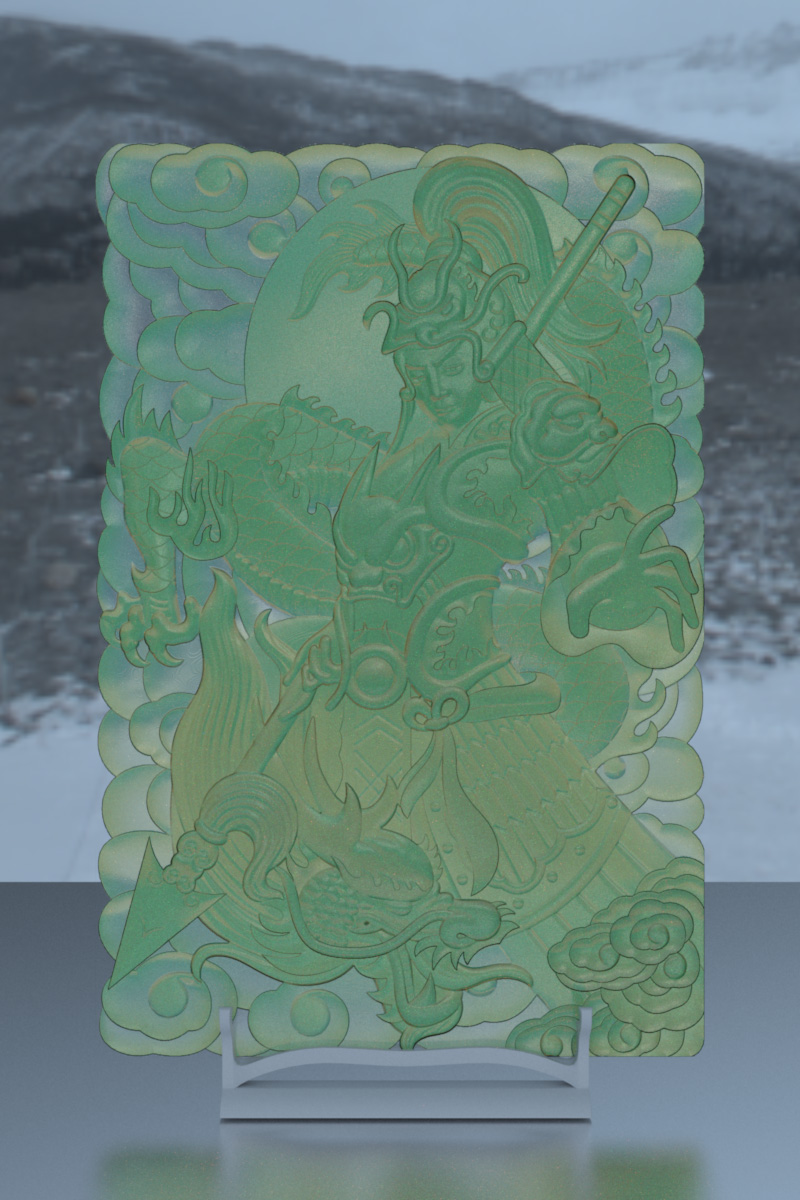
\includegraphics[width=\resLen]{layeredbsdf/results/zhaoyun_bg2_2.jpg}\\
		Back-lit & Front-lit & Back-lit & Front-lit
	\end{tabular}
	\caption[Reflection and transmission A]{\label{fig:layeredbsdf:zhaoyun}
		\textbf{Reflection and transmission:}
		A flat surface rendered with our layered BSDF under varying illuminations. This model involves dielectric interfaces with spatially varying roughnesses, normal maps, and thickness. The optical densities (mean free paths) are spectrally varying, which results in subtle color variations across the surface. Note that the color (albedo) is not varying.
	}
\end{figure}